\documentclass{article}
\usepackage[utf8]{inputenc}
\title{Video 2: the bootstrap}
\author{wbg231 }
\date{December 2022}
\newcommand{\R}{$\mathbb{R}$}
\newcommand{\B}{$\beta$}
\newcommand{\A}{$\alpha$}
\newcommand{\D}{\Delta}

\newcommand{\avector}[2]{(#1_2,\ldots,#1_{#2})}
\newcommand{\makedef}[2]{$\textbf{#1}$:#2 }
\usepackage{tikz,graphicx,hyperref,amsmath,amsfonts,amscd,amssymb,bm,cite,epsfig,epsf,url}

\begin{document}

\maketitle

\section{introduction}
\begin{itemize}
\item \href{https://www.youtube.com/watch?v=yeiMMzjDTWs&list=PLBEf5mJtE6KuZ5NBQMuWIMsiOOrV9ibzm&index=75}{video link}
\subsection{random sampling}
\item we want to estimate the average high in some population
\item we can not measure everyone so we just have a random  independent sample from the population and use that to estimate the population mean
\item the population mean is fixed, the sample mean is a random variable
\item the sample mean has a certain distribution that we can analyze
\subsection{confidence interval}
\item a range of values that contain the parameter 1-$\alpha$ percentage of the time 
\itme we know the population mean is distributed as a Gaussian with a certain mean and variance 
\item we can easily construct an area our on the pdf of that Gaussian that contains 95\% of the probability density
\item that requires us to understand the width of that interval, and center it at the sample mean
\subsection{standard error}
\item we have to estimate the width from the data, which we can do with standard error
\item for the sample mean we know that $se[\Tilde{m}]=\frac{\sigma_{pop}}{\sqrt{n}}$ \item we don't know $\sigma_{pop}$ but we can estimate it form our data with the sample standard deviation 
\item but notice that when constructing the confidence interval for a sample mean we knew the formula for the standard error, what happens if we do not have that formula?
\subsection{challenges}
\item how can we computationally estimate the standard errors 
\item if we could get more samples it would be really easy, we could just get many sample means and build the distribution of the sample means and estimate standard error but we cant do that obviously
\item we only have our one sample of n data points that is all we can use 
\item but what if we treated our n data as a population and used that to estimate the standard error 
\subsection{the bootstrap}
\item we have one sample $x_1..x_n$
\item we can make bootstrap indices $\Tilde{k}_1...\Tilde{k}_{n}$  
\item sampling independently and at random from the sample with replacement such that $P(\Tilde{k}_{j}=i)=\frac{1}{n}i,j\in[1,n]$
\item then we can create bootstrap samples $\Tilde{b}_1...\Tilde{b}_n$ such that $\Tilde{b}_j=X_{k,j}$ that is we are just taking bootstrap samples form our sample with replacement 
\item notice here that our sample is fixed but our bootstrap samples and indices are not 
\subsection{why called bootstrap}
\item the idea is you are pulling yourself up fro om your boots rap
\item it is something that should not work but does. 
\subsection{boots rap standard error}
\item we have samples$x_1..x_n$
\item we have our estimator $h(x_1..n)$
\item we have boots rap sample $\Tilde{b}_1,...\Tilde{b}_n$
\item the bootstrap standard error of h is $se_{bs}=\sqrt{var[h(\Tilde{b}_1....\Tilde{b}_n]}$
\item in order to compute this standard deviation we need to approximate using the monte carlo method
\subsection{monte carlo approx}
\item step 1. generate k boostrap samples $b_j^{k}$ of size n 
\item we compute the parameter estimate corresponding to each bootstrap  call the estimator from bootstrap i $w_i$ so we have $W=\{w_1..W_n\}$
\item step 3. bootstrap standard error: by taking the sample standard deviation of W, 
\item and use that to estimate our standard error of the populating just using the sample
\item we can take as many bootstraps as we would like 
\subsection{bootstrap samples}
\item look similar to the original sample, but because we are re sampling have some variance 
\item so what can we say about the distribution of the values of the bootstrap estimators
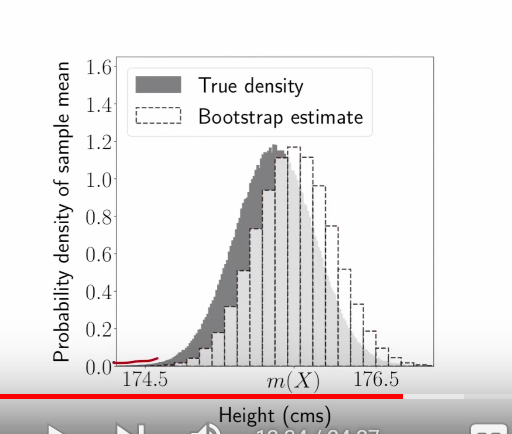
\includegraphics[width=10cm]{notes/week_5/video_2:the boostrap/immages/Screenshot 2023-02-25 at 23-34-20 Carlos Fernandez-Granda.png}
\item we an not completely estimate the true density form the boots rap samples, but we can get close dune rte right assumptions
\item further the width (which is the standard error) of the intervals are almost the same so it is a really good estimate of the standard error 
\subsection{traditional standard error estimate}
\item the bootstrap estimate and calculating the standard error with the formula is almost the same which is good 
\item why does this work 
\begin{itemize}
    \item we treat our sample as $X=x_1...x_n$ as the population
    \item the mean of each bootstrap is $m_{bs}=\frac{1}{n}\Sigma_{i=1}^{n}\Tilde{b}_k=m(X)$ that is the mean of our bootstraps means will be the sample mean 
    \item $se^2_{bs}=var[\Tilde{m}_{bs}]=\frac{\text{population variance}}{n}=\frac{\frac{1}{n}\Sigma_{i=1}^n(x_j-m(x))^2)}{n}=\frac{n-1}{n^2}V(X)$ so this is exactly the same as the sample standard error, and will approach the population sample error asymptotically
    \item so that is why the boots tap animates are shifted but the standard error are very close
\end{itemize}
\subsection{confidence interval for a Gaussian}
\item for $\Tilde{a}$ with mean $\mi$ and variance $\sigma^2$
\item the confidence interval is $\Tilde{I}=[\Tilde{a}-c_{\alpha}\sigma,\Tilde{a}+c_{\alpha}\sigma ]$
\subsection{boots tap Gaussian confidence interval}
\item sample $X=\{x_1...x_n\}$
\item h(X) is our estimator on the sample
\item bootstrap standard error $se_{bs}$
\item we can write a  $1-\alpha$ confidence interval  as $$\Tilde{I}_{1-\alpha}^{bs}=[h(X)-c_{1-\alpha}se_{bs},h(X)+c_{1-\alpha}se_{bs}]$$
\subsection{population correlation coefficient}
\item suppose we want to estimate the population correlating coefficient between foot Lent and height in a population 
\item we do not have an estimate for the standard error of the correlation coefficient so how do we get a standard error?
\item we can use the boostrap! and get an estimate of the standard error of the sample correlation coefficient over many bootstraps
\item this ends up doing really well
\item so our confidence interval of the correlation coefficient is $1-\alpha$ confidence interval  as $$\Tilde{I}_{1-\alpha}^{bs}=[\rho_{sample}-c_{1-\alpha}se_{bs},\rho_{sample}+c_{1-\alpha}se_{bs}]$$ under the assumption that the distribution of the estimator or Gaussian 
\item we can use this to build many confidence intervals, and try to see if it 
\item this is nice because we no longer need the formula for the standard error of our estimator as long as the estimator is distributed Gaussian 
\end{itemize}
\end{document}
